\documentclass[../../../../main.tex]{subfiles}
\begin{document}

平面上に点 $O$ を中心とする半径1の円 $C$ がある．
また，この平面上の $O$ と異なる点 $A$ を通って直線 $OA$ と垂直な空間直線 $\ell$ があり，
平面とのなす角が $45^\circ$ である．
このとき，円 $C$ と直線 $\ell$ の間の最短距離を，2点 $O$，$A$ 間の距離 $a$ で表せ．

\begin{figure}[htbp]
  \centering
  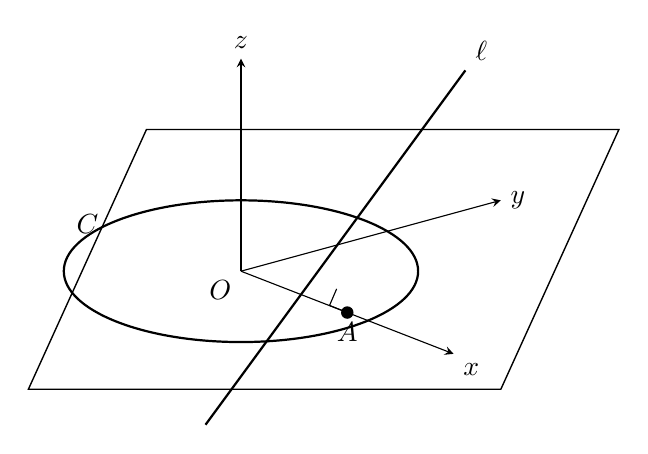
\begin{tikzpicture}[scale=1.5, >=stealth]
    \draw[line width=0.5pt] (-1.8,-1.0) -- (2.2,-1.0) -- (3.2,1.2) -- (-0.8,1.2) -- cycle;

    \draw[->] (0,0) -- (1.8,-0.7) node[below right] {$x$};
    \draw[->] (0,0) -- (2.2,0.6) node[right] {$y$};
    \draw[->] (0,0) -- (0, 1.8) node[above] {$z$};
    \node[below left] at (0,0) {$O$};

    \draw[thick] (0,0) ellipse (1.5 and 0.6);
    \node at (-1.3, 0.4) {$C$};

    \coordinate (A) at (0.9, -0.35);
    \fill (A) circle (1.5pt) node[below] {$A$};

    \draw[thick] (-0.3, -1.3) -- (1.9, 1.7) node[above right] {$\ell$};

    \draw (0.9, -0.35) -- (0.75, -0.29) -- (0.81, -0.15);
  \end{tikzpicture}
\end{figure}

\end{document}
